% Options for packages loaded elsewhere
\PassOptionsToPackage{unicode}{hyperref}
\PassOptionsToPackage{hyphens}{url}
%
\documentclass[
  man,floatsintext]{apa6}
\usepackage{amsmath,amssymb}
\usepackage{lmodern}
\usepackage{iftex}
\ifPDFTeX
  \usepackage[T1]{fontenc}
  \usepackage[utf8]{inputenc}
  \usepackage{textcomp} % provide euro and other symbols
\else % if luatex or xetex
  \usepackage{unicode-math}
  \defaultfontfeatures{Scale=MatchLowercase}
  \defaultfontfeatures[\rmfamily]{Ligatures=TeX,Scale=1}
\fi
% Use upquote if available, for straight quotes in verbatim environments
\IfFileExists{upquote.sty}{\usepackage{upquote}}{}
\IfFileExists{microtype.sty}{% use microtype if available
  \usepackage[]{microtype}
  \UseMicrotypeSet[protrusion]{basicmath} % disable protrusion for tt fonts
}{}
\makeatletter
\@ifundefined{KOMAClassName}{% if non-KOMA class
  \IfFileExists{parskip.sty}{%
    \usepackage{parskip}
  }{% else
    \setlength{\parindent}{0pt}
    \setlength{\parskip}{6pt plus 2pt minus 1pt}}
}{% if KOMA class
  \KOMAoptions{parskip=half}}
\makeatother
\usepackage{xcolor}
\usepackage{graphicx}
\makeatletter
\def\maxwidth{\ifdim\Gin@nat@width>\linewidth\linewidth\else\Gin@nat@width\fi}
\def\maxheight{\ifdim\Gin@nat@height>\textheight\textheight\else\Gin@nat@height\fi}
\makeatother
% Scale images if necessary, so that they will not overflow the page
% margins by default, and it is still possible to overwrite the defaults
% using explicit options in \includegraphics[width, height, ...]{}
\setkeys{Gin}{width=\maxwidth,height=\maxheight,keepaspectratio}
% Set default figure placement to htbp
\makeatletter
\def\fps@figure{htbp}
\makeatother
\setlength{\emergencystretch}{3em} % prevent overfull lines
\providecommand{\tightlist}{%
  \setlength{\itemsep}{0pt}\setlength{\parskip}{0pt}}
\setcounter{secnumdepth}{-\maxdimen} % remove section numbering
% Make \paragraph and \subparagraph free-standing
\ifx\paragraph\undefined\else
  \let\oldparagraph\paragraph
  \renewcommand{\paragraph}[1]{\oldparagraph{#1}\mbox{}}
\fi
\ifx\subparagraph\undefined\else
  \let\oldsubparagraph\subparagraph
  \renewcommand{\subparagraph}[1]{\oldsubparagraph{#1}\mbox{}}
\fi
\newlength{\cslhangindent}
\setlength{\cslhangindent}{1.5em}
\newlength{\csllabelwidth}
\setlength{\csllabelwidth}{3em}
\newlength{\cslentryspacingunit} % times entry-spacing
\setlength{\cslentryspacingunit}{\parskip}
\newenvironment{CSLReferences}[2] % #1 hanging-ident, #2 entry spacing
 {% don't indent paragraphs
  \setlength{\parindent}{0pt}
  % turn on hanging indent if param 1 is 1
  \ifodd #1
  \let\oldpar\par
  \def\par{\hangindent=\cslhangindent\oldpar}
  \fi
  % set entry spacing
  \setlength{\parskip}{#2\cslentryspacingunit}
 }%
 {}
\usepackage{calc}
\newcommand{\CSLBlock}[1]{#1\hfill\break}
\newcommand{\CSLLeftMargin}[1]{\parbox[t]{\csllabelwidth}{#1}}
\newcommand{\CSLRightInline}[1]{\parbox[t]{\linewidth - \csllabelwidth}{#1}\break}
\newcommand{\CSLIndent}[1]{\hspace{\cslhangindent}#1}
\ifLuaTeX
\usepackage[bidi=basic]{babel}
\else
\usepackage[bidi=default]{babel}
\fi
\babelprovide[main,import]{english}
% get rid of language-specific shorthands (see #6817):
\let\LanguageShortHands\languageshorthands
\def\languageshorthands#1{}
% Manuscript styling
\usepackage{upgreek}
\captionsetup{font=singlespacing,justification=justified}

% Table formatting
\usepackage{longtable}
\usepackage{lscape}
% \usepackage[counterclockwise]{rotating}   % Landscape page setup for large tables
\usepackage{multirow}		% Table styling
\usepackage{tabularx}		% Control Column width
\usepackage[flushleft]{threeparttable}	% Allows for three part tables with a specified notes section
\usepackage{threeparttablex}            % Lets threeparttable work with longtable

% Create new environments so endfloat can handle them
% \newenvironment{ltable}
%   {\begin{landscape}\centering\begin{threeparttable}}
%   {\end{threeparttable}\end{landscape}}
\newenvironment{lltable}{\begin{landscape}\centering\begin{ThreePartTable}}{\end{ThreePartTable}\end{landscape}}

% Enables adjusting longtable caption width to table width
% Solution found at http://golatex.de/longtable-mit-caption-so-breit-wie-die-tabelle-t15767.html
\makeatletter
\newcommand\LastLTentrywidth{1em}
\newlength\longtablewidth
\setlength{\longtablewidth}{1in}
\newcommand{\getlongtablewidth}{\begingroup \ifcsname LT@\roman{LT@tables}\endcsname \global\longtablewidth=0pt \renewcommand{\LT@entry}[2]{\global\advance\longtablewidth by ##2\relax\gdef\LastLTentrywidth{##2}}\@nameuse{LT@\roman{LT@tables}} \fi \endgroup}

% \setlength{\parindent}{0.5in}
% \setlength{\parskip}{0pt plus 0pt minus 0pt}

% Overwrite redefinition of paragraph and subparagraph by the default LaTeX template
% See https://github.com/crsh/papaja/issues/292
\makeatletter
\renewcommand{\paragraph}{\@startsection{paragraph}{4}{\parindent}%
  {0\baselineskip \@plus 0.2ex \@minus 0.2ex}%
  {-1em}%
  {\normalfont\normalsize\bfseries\itshape\typesectitle}}

\renewcommand{\subparagraph}[1]{\@startsection{subparagraph}{5}{1em}%
  {0\baselineskip \@plus 0.2ex \@minus 0.2ex}%
  {-\z@\relax}%
  {\normalfont\normalsize\itshape\hspace{\parindent}{#1}\textit{\addperi}}{\relax}}
\makeatother

% \usepackage{etoolbox}
\makeatletter
\patchcmd{\HyOrg@maketitle}
  {\section{\normalfont\normalsize\abstractname}}
  {\section*{\normalfont\normalsize\abstractname}}
  {}{\typeout{Failed to patch abstract.}}
\patchcmd{\HyOrg@maketitle}
  {\section{\protect\normalfont{\@title}}}
  {\section*{\protect\normalfont{\@title}}}
  {}{\typeout{Failed to patch title.}}
\makeatother

\usepackage{xpatch}
\makeatletter
\xapptocmd\appendix
  {\xapptocmd\section
    {\addcontentsline{toc}{section}{\appendixname\ifoneappendix\else~\theappendix\fi\\: #1}}
    {}{\InnerPatchFailed}%
  }
{}{\PatchFailed}
\keywords{heart rate; photoplethysmography; wearable electronic device; teaching\newline\indent Word count: X}
\usepackage{lineno}

\linenumbers
\usepackage{csquotes}
\ifLuaTeX
  \usepackage{selnolig}  % disable illegal ligatures
\fi
\IfFileExists{bookmark.sty}{\usepackage{bookmark}}{\usepackage{hyperref}}
\IfFileExists{xurl.sty}{\usepackage{xurl}}{} % add URL line breaks if available
\urlstyle{same} % disable monospaced font for URLs
\hypersetup{
  pdftitle={New approaches to teachers' experience of stress: Do heart rate measurements with fitness trackers provide an efficient, inexpensive, and robust measurement method?},
  pdfauthor={Mandy Klatt1, Peer Keßler1, Gregor Kachel1,2, Christin Lotz1, \& Anne Deiglmayr1},
  pdflang={en-EN},
  pdfkeywords={heart rate; photoplethysmography; wearable electronic device; teaching},
  hidelinks,
  pdfcreator={LaTeX via pandoc}}

\title{New approaches to teachers' experience of stress: Do heart rate measurements with fitness trackers provide an efficient, inexpensive, and robust measurement method?}
\author{Mandy Klatt\textsuperscript{1}, Peer Keßler\textsuperscript{1}, Gregor Kachel\textsuperscript{1,2}, Christin Lotz\textsuperscript{1}, \& Anne Deiglmayr\textsuperscript{1}}
\date{}


\shorttitle{Using fitbit to measure teachers' heart rate}

\authornote{

We received funding from QualiFond of University Leipzig. We have no conflicts of interest to disclose. This article is based on data used at conference presentations (DACH-Nachwuchsakademie, 2022; EARLI SIG 11, 2022; EARLI SIG 27, 2022).

The authors made the following contributions. Mandy Klatt: Conceptualization, Writing - Original Draft Preparation, Writing - Review \& Editing; Peer Keßler: Writing - Original Draft Preparation, Writing - Review \& Editing; Gregor Kachel: Conceptualization, Writing - Original Draft Preparation, Writing - Review \& Editing; Christin Lotz: Conceptualization, Writing - Original Draft Preparation, Writing - Review \& Editing; Anne Deiglmayr: Supervision.

Correspondence concerning this article should be addressed to Mandy Klatt, Dittrichring 5-7, 04109 Leipzig. E-mail: \href{mailto:mandy.klatt@uni-leipzig.de}{\nolinkurl{mandy.klatt@uni-leipzig.de}}

}

\affiliation{\vspace{0.5cm}\textsuperscript{1} Leipzig University\\\textsuperscript{2} Max Planck Institute for Evolutionary Anthropology}

\abstract{%
One or two sentences providing a \textbf{basic introduction} to the field, comprehensible to a scientist in any discipline.

Two to three sentences of \textbf{more detailed background}, comprehensible to scientists in related disciplines.

One sentence clearly stating the \textbf{general problem} being addressed by this particular study.

One sentence summarizing the main result (with the words ``\textbf{here we show}'' or their equivalent).

Two or three sentences explaining what the \textbf{main result} reveals in direct comparison to what was thought to be the case previously, or how the main result adds to previous knowledge.

One or two sentences to put the results into a more \textbf{general context}.

Two or three sentences to provide a \textbf{broader perspective}, readily comprehensible to a scientist in any discipline.

XXX In this proof-of-concept study, we aimed to advance the field of teacher stress by collecting heart rate data with wrist-worn devices and testing a methodology that has the potential to provide more insights on the non-invasive assessment of teacher stress. XXX
}



\begin{document}
\maketitle

\hypertarget{introduction}{%
\section{Introduction}\label{introduction}}

Physiological data such as heart rate are becoming increasingly important in research on stress experience. They represent an important indicator of physical or emotional stress, as increased workload is associated with increased heart rate (Sachs, 2014). Furthermore, they allow a more objective recording of stress than self-reports (Runge, Haarman, \& Fisher, n.d.). However, capturing heart rate in an educational context requires the use of low-cost and non-invasive instruments. Fitness trackers worn on the wrist have the potential to be such a useful tool (Ferguson, Rowlands, Olds, \& Maher, 2015).

To date, there is still little evidence on the usefulness of heart rate measurements using fitness trackers in teaching and learning settings (Ertzberger \& Martin, 2016; Lowe, 2016). Runge et al. (n.d.) alone examined teacher stress in a relatively small sample (\emph{N} = 4 teachers) and showed that high heart rate indicates more stress in teachers.

Thus, there remains a lack of robust studies on whether fitness trackers are an efficient, low-cost, and robust measurement method for assessing teachers' experience of arousal during teaching.

\hypertarget{theoretical-background}{%
\section{Theoretical Background}\label{theoretical-background}}

\hypertarget{stress-in-teaching-profession}{%
\subsection{Stress in Teaching Profession}\label{stress-in-teaching-profession}}

--\textgreater{} teacher profession is one of the most stressful professions.

Teacher stress can be defined as ``{[}\ldots{]} the experience by a teacher of unpleasant, negative emotions, such as anger, anxiety, tension, frustration or depression, resulting from some aspect of their work as a teacher.'' (Kyriacou, 2001).

Teachers' individual perceptions of student misbehavior in the classroom are closely related to their well-being (Aldrup, Klusmann, Lüdtke, Göllner, \& Trautwein, 2018).

--\textgreater{} wie entsteht Stress

--\textgreater{} wie wurde Stress bisher gemessen

\hypertarget{heart-rate-as-an-indicator-for-stress-or-arousal}{%
\subsection{Heart rate as an indicator for stress or arousal}\label{heart-rate-as-an-indicator-for-stress-or-arousal}}

Heart rate is physiologically regulated by the autonomic nervous system. An increase in the activity of the sympathetic as part of the autonomic nervous system results in the heart rate being speeded up (``fight or flight''). On the other hand, an increased activity of the parasympathetic as the counterpart has the effect of slowing down the heart rate (``rest and digest'') (Battipaglia \& Lanza, 2015). In addition to the autonomic nervous system and genetic factors, heart rate is influenced by numerous external factors such as social, personal, psychological, environmental and behavioural factors (Wang, Lizardo, \& Hachen, 2022).

\hypertarget{wrist-worn-devices-as-a-new-approach-to-assess-physiological-measures}{%
\subsection{Wrist-worn devices as a new approach to assess physiological measures}\label{wrist-worn-devices-as-a-new-approach-to-assess-physiological-measures}}

Fuller et al. (2020) showed in their review article that wearable devices such as Fitbit watches are accurate and reliable for measuring heart rate in controlled settings.

``The use of physiological measures enabled us to get some insight into teachers' affective responses without disrupting the teaching process (Mauss \& Robinson, 2009) and to reduce issues with social desirability, retrospective bias, and high cognitive load (Becker et al., 2015; Goetz et al., 2015; Scollon et al.,2009; Wilhelm \& Grossman, 2010). Moreover, we found that heart rate measures discriminated between both teachers, even when their interpersonal behavior during the lesson start was relatively similar.''

\begin{enumerate}
\def\labelenumi{(\arabic{enumi})}
\setcounter{enumi}{19}
\tightlist
\item
  (PDF) A Quantitative Exploration of Two Teachers with Contrasting Emotions: Intra-Individual Process Analyses of Physiology and Interpersonal Behavior. Available from: \url{https://www.researchgate.net/publication/329787434_A_Quantitative_Exploration_of_Two_Teachers_with_Contrasting_Emotions_Intra-Individual_Process_Analyses_of_Physiology_and_Interpersonal_Behavior} {[}accessed Dec 07 2022{]}.
\end{enumerate}

\hypertarget{aim-of-the-study}{%
\subsection{Aim of the study}\label{aim-of-the-study}}

In the present study, we assessed HR measures and self-report data of pre- and in-service teachers in a controlled teaching-learning setting. The aim was to investigate whether heart rate measurements using wrist-worn fitness trackers are a suitable and effective method \textbf{(1)} to map differences in states of arousal between five different phases (pre-teaching phase, teaching phase, post-teaching phase, interview phase and end phase) and \textbf{(2)} to evaluate the correlation between self-reported evaluations and HR measures.

\textbf{(H1)} We expected heart rates to be higher during the teaching phase than during the pre- and the three post-teaching phases, and that the HR measures would decrease over the course of the study. \textbf{(H2)} We also predicted that HR and a high ranking on the negative scale on our survey (feeling disturbed by disruptions) would correlate positively and a high ranking on the positive scale (feeling confident in dealing with disruptions) would follow the inverse pattern.

\hypertarget{methods}{%
\section{Methods}\label{methods}}

We report how we determined our sample size, all data exclusions (if any), all manipulations, and all measures in the study.

\hypertarget{participants}{%
\subsection{Participants}\label{participants}}

The sample consisted in total of \emph{N} = 63 pre- and in-service teachers. The subjects were recruited from the Leipzig University or from German schools in Saxony via personal contact, e-mail lists and flyers. Data of two participants were excluded from the analyses due to insufficient data quality, yielding data from \emph{N} = 61 subjects.

The subjects (39 women; 63.93 \%) had a mean age of 29.60 years (\emph{SD} = 10.40; range: 19-59) and an average teaching experience of 4.66 years (\emph{SD} = 9.30; range: 0-37).

18.03\% of the subjects were (studying to become) teachers for primary school, 72.13\% were (studying to become) teachers for secondary school and 9.84\% were (studying to become) teachers for special education needs.

All study procedures were carried out in accordance with the ethical standards of the University's Institutional Review Board and the authors received a positive vote on the study procedures from the Ethics Committee Board of Leipzig University. All participants were informed in detail about the aim and intention of the study prior to testing. Participation in the study was voluntary and only took place after written consent has been given.

\hypertarget{material}{%
\subsection{Material}\label{material}}

\hypertarget{teachers-heart-rate}{%
\subsubsection{Teachers' heart rate}\label{teachers-heart-rate}}

We used a Fitbit Charge 4 to measure the teachers' heart rate. The device was attached 2-finger widths above the ulnar styloid process to the subject's wrist following the manufacturer's instructions. To determine the heart rate, the Fitbit flashes green LEDs many times per second and uses light-sensitive photodiodes to measure the volume changes in the capillaries and then calculates how many times the heart beats per minute (bpm). Data were automatically wireless synced with an iPad via Bluetooth to a Fitbit account, and subsequently, the intraday second-by-second data were exported for each session using the opensource software Pulse Watch (PulseWatch. URL: \url{https://iccir919.github.io/pulseWatch/public/index.html} {[}accessed 2022-08-03{]}).

\hypertarget{teachers-self-reported-data-of-arousal-during-the-teaching-phase}{%
\subsubsection{Teachers' self-reported data of arousal during the teaching phase}\label{teachers-self-reported-data-of-arousal-during-the-teaching-phase}}

The subject's self-reported data of arousal in response to the nine disruptions during the lesson was assessed in a Stimulated Recall Interview that took place after the lesson. For this purpose, two numerical 11-point rating scales were used: \emph{(1)} The first rating scale collected data of the teacher's subjective perception of disruptiveness of each disruption (``On a scale of 0-10: how disruptive did you find the event? 0 is not disruptive at all, 10 is extremely disruptive'') \emph{(2)} The second rating scale assessed the teacher's subjective perception of confidence in dealing with the disruptions during the lesson (``How confident did you feel in dealing with this event on a scale of 0-10? 0 is not confident at all and 10 is extremely confident'').

The response format was purposely chosen to be closed and with several answer options in order to assign numerical values to the subjects' self-report and emotional experience, and thus to make them measurable and comparable (Döring \& Bortz, 2016; Eid, Gollwitzer, \& Schmitt, 2015). The gradations of the rating scale were unambiguous and the intervals between them identical. The characteristic value was estimated by the subjects immediately after seeing the recording of the respective disruption and communicated verbally to the experimenter.

\hypertarget{procedure}{%
\subsection{Procedure}\label{procedure}}

The data collection was part of a larger research project with a planned sample of \emph{n} = 40 in-service teachers and \emph{n} = 40 pre-service teachers.

The study took place in the rooms of the Faculty of Education at Leipzig University. In a controlled laboratory setting, heart rate data in beats per minute (bpm) were recorded using Fitbit Charge 4 over a total period of approximately two hours. Within this time frame, teachers taught a 15-minute self-prepared lesson to an audience of three actors.

For this purpose, a seminar room was converted into a classroom. The classroom was equipped with a digital whiteboard and a blackboard. The fictitious class consisting of three trained actors sat facing the teacher head-on in a ``U''; pen and paper were provided on their seats. In addition, the students brought their own mobile phone, which was also visibly positioned on the desk.

The subject was instructed during the lesson to behave and move as naturally as possible, as they would in a real classroom. In advance, all subjects were given information about planning their lesson in a meeting to ensure that an appropriately realistic teaching situation could take place, e.g.~it was pointed out that longer film clips as well as group work as a social form should be avoided in order to ensure interaction between teacher and students in the short time of the study.

For analyzing the heart rate data, we focused on five 10-minute intervals of theoretical interest for multiple reason. First, 10 minutes was to the minimum duration of all intervals, so we wanted to ensure the comparability of the intervals for all participants. Second, Lu et al. (2008) confirmed in their study that 10-minute intervals are an useful duration for analyzing photoplethysmography (PPG) data. Third, other studies revealed that the first minutes of the lesson start are essential regarding teacher-student interaction (Claessens et al., 2017; Donker, Van Gog, \& Mainhard, 2018).

The procedure of the study and how we calculated the five phases is described in the following:

\emph{(1)} The \emph{pre-teaching phase} was the first 10-minute interval of interest. This interval was calculated from the moment the subject arrived and the Fitbit watch was put on, which happened immediately after the subject was welcomed by the experimenter and the three actors. After the experimenter briefly explained the project and the procedure of the study to the subject, contact details were subsequently collected as part of the hygiene concept of COVID-19 and the written consent to voluntarily participate in the study was requested. Next, the subject was asked to prepare the necessary materials for the lesson (connecting the laptop to the beamer, preparing worksheets, etc.). This phase varied in duration according to the prepared lesson (about 1-5min on average).

Once the preparation was completed, the eye-tracking glasses were briefly explained to the subject as well as the adjustment made to the subject by the experimenter (changing the lenses or the nose pad if necessary). Subsequently, a 1-point calibration of the eye-tracking glasses took place and together with further devices (GoPro camera, 3D camera, audio recorder) the recordings were started.

Before the lesson began, a warm-up phase took place to familiarize the subject with the laboratory setting and equipment. This warm-up phase consisted of two parts:

\begin{itemize}
\tightlist
\item
  In the first part, the subject and the three actors playfully learned each other's names. Additional fictitious name tags of the actors were attached to the table and did not change across the study. In the game, by throwing two balls, either the participant's own name or the name of the target person was called.
\item
  The second part of the warm-up phase involved getting into conversation with each other by asking questions. For this purpose, the subject was asked to come up with a question for each of the actors (three questions in total) and was also asked a question in return by each actor. This could be anything that interested the participants. The questions should be as authentic as possible and were not tailored to the role of the actors.
  The purpose of this warming-up phase was, on the one hand, to make the subject forget about the devices and, on the other hand, to create as realistic as possible a classroom situation in which interactions were based on a teacher-student relationship.
\end{itemize}

The pre-teaching phase lasted 10-15 minutes on average, depending on different issues (preparing the lesson, technical problems, adjusting the eye-tracking glasses).

\emph{(2)} The second 10-minute interval was the \emph{teaching phase}, which began with the experimenter noting the time and step count of the fitness tracker. The subject was then asked to carry out a 9-point calibration alone in a room next door. After the calibration, the lesson started with the subject opening the door to the laboratory room.
During the lesson, the actors were instructed to simulate nine typical classroom events, three each in the following categories: (a) verbal disruptive behavior (chatting with the neighbor, whispering, heckling), (b) physical disruptions (clicking with a pen, drumming with hands on the table, snipping) and (c) lack of eagerness to learn (drawing on a sheet of paper, putting the head on the table, looking at the phone).

The order of the events and the performing actors were fully balanced with Latin square. The actors were trained before to perform the disruptions identically in each data collection.

After a short familiarization phase for the teacher of two and a half minutes, the instructions appeared as intervals (every 90 seconds for 30 seconds) on a screen that was only visible for the class. The actors were trained to stop the disruptive behavior as soon as the teacher intervened.

Time management was regulated by the experimenter by showing time cards (yellow = 1 minute until the end; red = end of the lesson). The lesson lasted about 18 minutes on average but only the first 10 minutes were used as an interval to ensure the identical duration for all participants. At the end of the lesson, the experimenter again noted the time and the steps on the clock.

\emph{(3)} The noted time of the lesson end was also the starting point for the \emph{post-teaching} phase as the third 10-minute interval. At the end of the lesson, the experimenter attached letters A through D in the lab while the teacher performed a second 9-point calibration outside. The letter search as a control condition was part of another project, which is why it will not be discussed further in the study. Subsequently, the subjects as well as the actors were given a short questionnaire, which contained items to collect demographic information as well as items about the previously given lesson on teaching quality (4-point Likert scale; 1 = strongly disagree; 2 = disagree; 3 = agree; 4 = strongly agree; EMU, Helmke et al. (2014)) via the online survey website SoSci Survey. The completion of the questionnaire took approximately 5 minutes.

Meanwhile, the experimenter prepared the second part of the data collection: The Stimulated Recall Interview. Within post-teaching phase, the majority of subjects completed the questionnaire and positioned themselves next to the experimenter to begin the interview. In some cases, the beginning of the interview was part of the post-teaching phase due to individual needs (going to the toilet, spending more time completing the questionnaire, etc.).

\emph{(4)} The fourth 10-minute interval of interest was the \emph{interview phase} that was 10 minutes in the middle of the interview. To ensure that all subjects were in the middle of the interview, we calculated the difference from the end of the lesson and from the time when the subject took off the watch. This duration was divided in two to get to the middle of the interval. Then, 5 minutes were subtracted to get to the start of the 10-minute interval.

The interview itself took place using the Think Aloud procedure (Konrad, 2020). For this purpose, the eye tracking video was watched again and the experimenter stopped the video at the nine disruptions when they appeared to asks several questions. The questions were identical for each disruption, they were asked in a fixed order.
First, the subject was asked to describe the disruption, to evaluate (11-point rating scale) and justify the disruptiveness of each disruption. Next, the subject was asked to describe and justify the reaction. The experimenter then asked the subject to evaluate (11-point rating scale) and justify the confidence the subject had in dealing with the disruption. Statements about the evaluation of the disruptiveness and the confidence were quantified. For this purpose, subjects determined their individual value on a rating scale from 0 (not disturbing / not safe) to 10 (disturbing / safe).

The interview lasted on average 45-60 minutes.

\emph{(5)} The last interesting interval for the analyses was the \emph{end phase}, which was the 10 minutes before the subject took off the watch. In this interval, the subject answered a second questionnaire (Situational Judgment Test, Gold and Holodynski (2015)) to assess the subject's strategic knowledge of classroom management. The subject was asked to judge alternative actions on school scenarios on a 6-point rating scale from 1 (A) to 6 (F) according to school grades. Data from the questionnaire were again collected as an online questionnaire via the website www.soscisurvey.de and lasted approximately 10-15 minutes.

The Fitbit watch was removed only after the last questionnaire to obtain heart rate data during the entire study.

\hypertarget{data-analysis}{%
\subsection{Data analysis}\label{data-analysis}}

We used R (Version 4.1.3; R Core Team, 2022) and the R-packages \emph{broom} (Version 1.0.1; Robinson, Hayes, \& Couch, 2022), \emph{cowplot} (Version 1.1.1; Wilke, 2020), \emph{DescTools} (Version 0.99.45; Andri et mult. al., 2022), \emph{dplyr} (Version 1.0.10; Wickham, François, Henry, \& Müller, 2022), \emph{forcats} (Version 0.5.1; Wickham, 2021), \emph{ggplot2} (Version 3.3.5; Wickham, 2016), \emph{ggpubr} (Version 0.4.0; Kassambara, 2020), \emph{ggthemes} (Version 4.2.4; Arnold, 2021), \emph{gridExtra} (Version 2.3; Auguie, 2017), \emph{imputeTS} (Version 3.2; Moritz \& Bartz-Beielstein, 2017), \emph{janitor} (Version 2.1.0; Firke, 2021), \emph{jtools} (Version 2.2.0; Long, 2022), \emph{lm.beta} (Version 1.6.2; Behrendt, 2022), \emph{lme4} (Version 1.1.30; Bates, Mächler, Bolker, \& Walker, 2015), \emph{ltm} (Version 1.2.0; Rizopoulos, 2006), \emph{lubridate} (Version 1.8.0; Grolemund \& Wickham, 2011), \emph{MASS} (Version 7.3.55; Venables \& Ripley, 2002), \emph{Matrix} (Version 1.5.1; Bates, Maechler, \& Jagan, 2022), \emph{msm} (Version 1.6.9; Jackson, 2011), \emph{needs} (Version 0.0.3; Katz, 2016), \emph{papaja} (Version 0.1.0.9999; Aust \& Barth, 2020), \emph{polycor} (Version 0.8.1; Fox, 2022), \emph{ppcor} (Version 1.1; Kim, 2015), \emph{purrr} (Version 0.3.4; Henry \& Wickham, 2020), \emph{readr} (Version 2.1.3; Wickham, Hester, \& Bryan, 2022), \emph{readxl} (Version 1.4.0; Wickham \& Bryan, 2022), \emph{rstatix} (Version 0.7.0; Kassambara, 2021), \emph{stringr} (Version 1.4.0; Wickham, 2019), \emph{tibble} (Version 3.1.6; Müller \& Wickham, 2021), \emph{tidyr} (Version 1.2.0; Wickham \& Girlich, 2022), \emph{tidyverse} (Version 1.3.1; Wickham et al., 2019), \emph{tinylabels} (Version 0.2.3; Barth, 2022), \emph{viridis} (Version 0.6.2; Garnier et al., 2021a, 2021b), \emph{viridisLite} (Version 0.4.1; Garnier et al., 2021b), and \emph{xfun} (Version 0.36; Xie, 2022) for all our analyses (descriptive statistics, correlations, and multilevel regression). Statistical assumptions including linearity, homogeneity of variance, and normal distribution of residuals were tested and confirmed with RStudio {[}palmeri2020{]}. An alpha level of 0.05 was used for the statistical tests.

\hypertarget{descriptive-statistics}{%
\subsubsection{Descriptive statistics}\label{descriptive-statistics}}

Means, standard deviations and the range of teachers' heart rate and the self-reported data are shown in Table 2.

Teachers' average heart rate during the entire course of the study was approximately 96.26 bpm with a standard deviation of 14.22 and a range from 56 to 139 bpm.

Means, standard deviations and the range of teachers' heart rate for the different phases and the self-reported data are shown in Table 2.

\hypertarget{pairwaise-t-test-and-effect-size}{%
\subsubsection{Pairwaise t-test and effect size}\label{pairwaise-t-test-and-effect-size}}

\hypertarget{multilevel-regressions}{%
\subsubsection{Multilevel regressions}\label{multilevel-regressions}}

XXX

\hypertarget{results}{%
\section{Results}\label{results}}

\hypertarget{first-visual-results}{%
\section{First visual results}\label{first-visual-results}}

The graph @ref(fig:overall\_plot) show the heart rate for the entire course of the study.

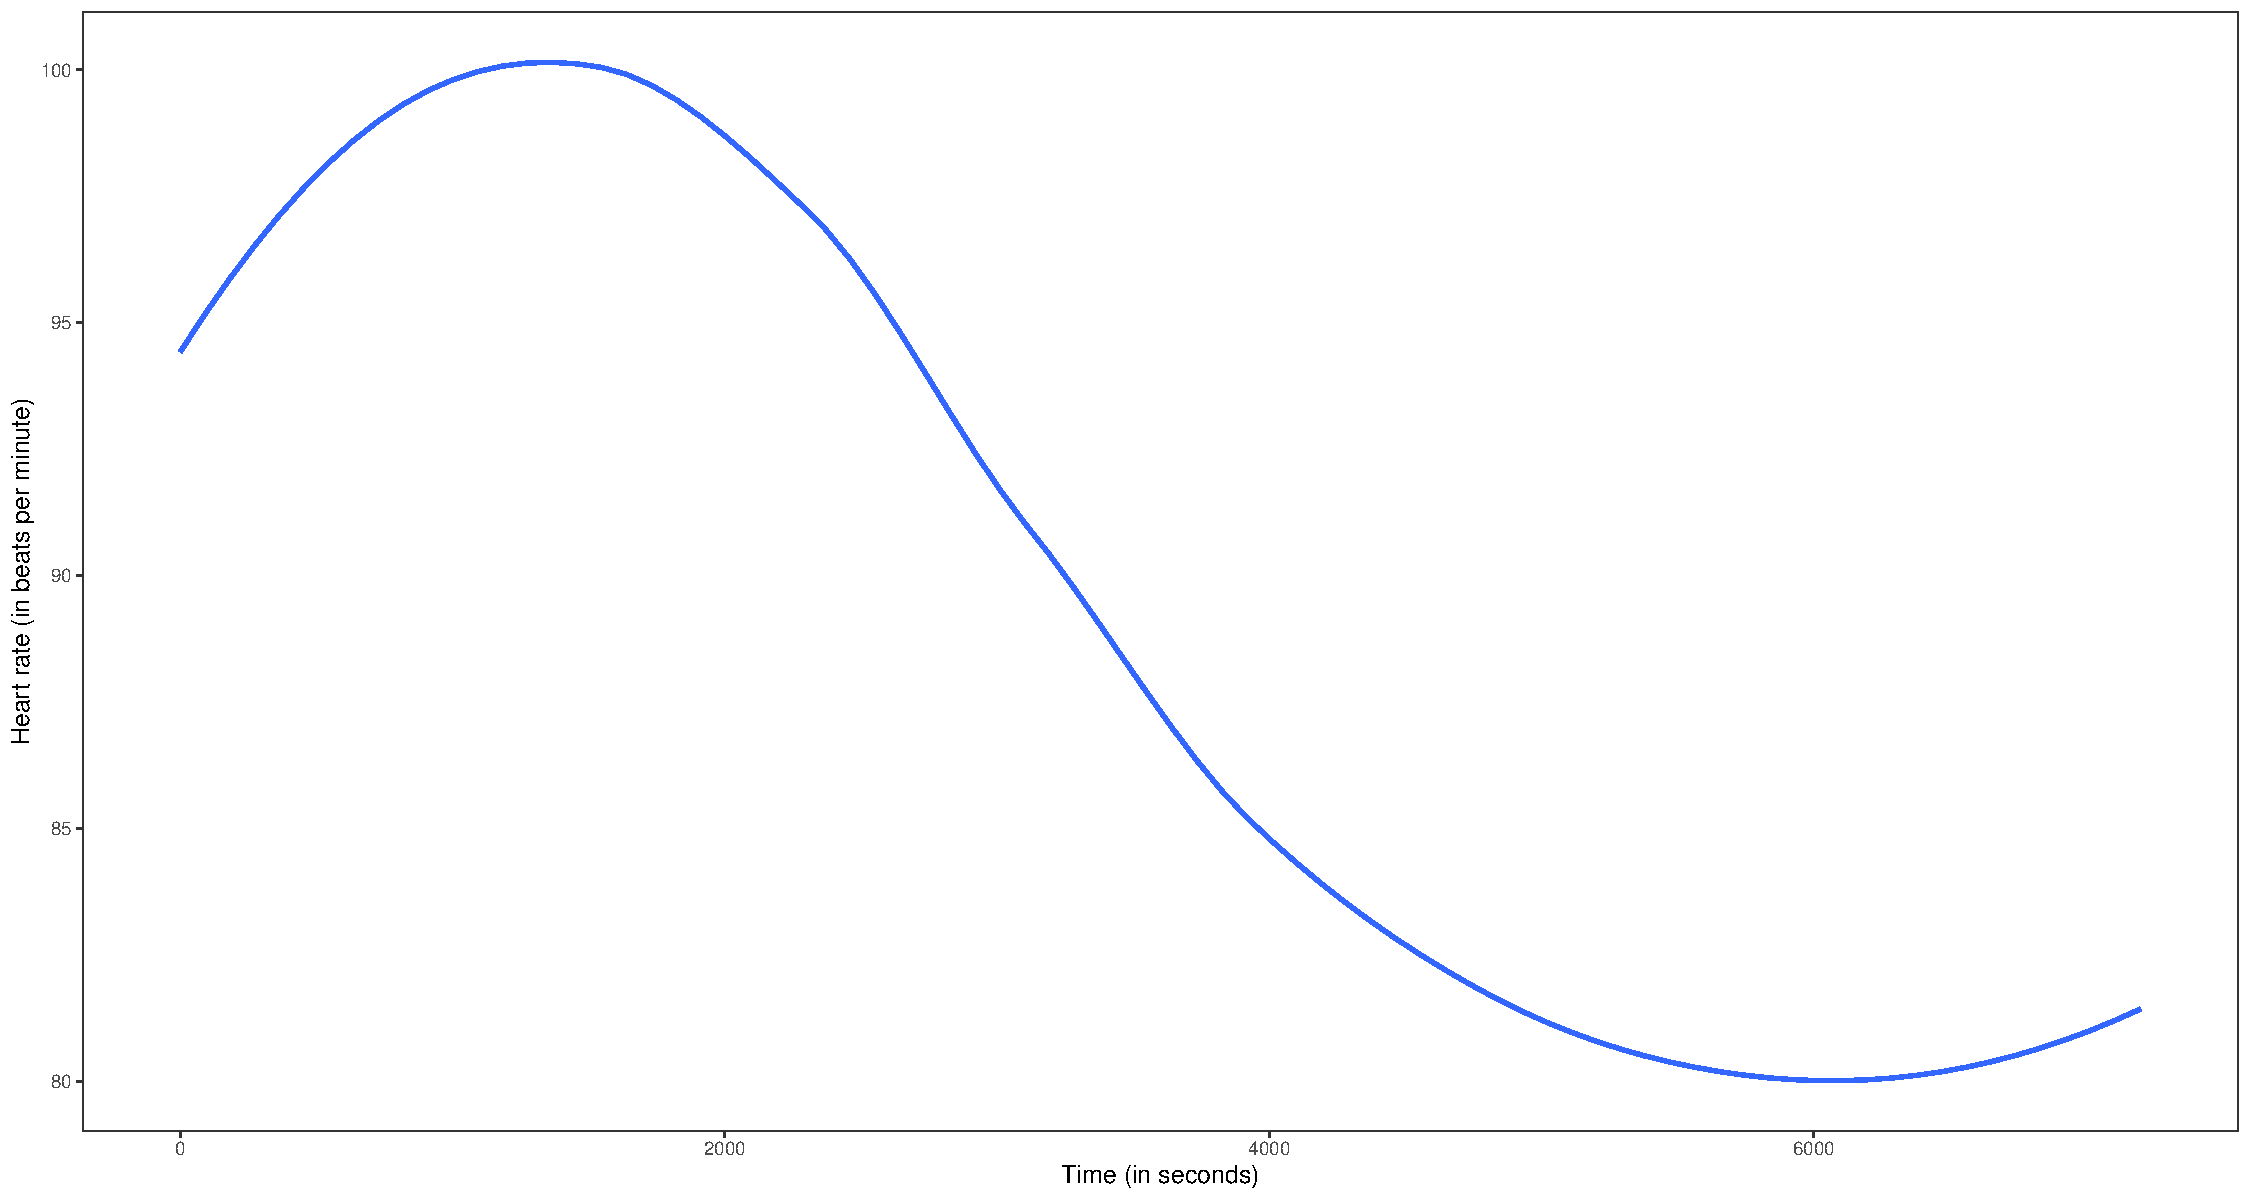
\includegraphics{fitbit_paper_files/figure-latex/overall_plot-1.pdf}

The second graph @ref(fig:phase\_plot) show the heart rate for the individual five phases.

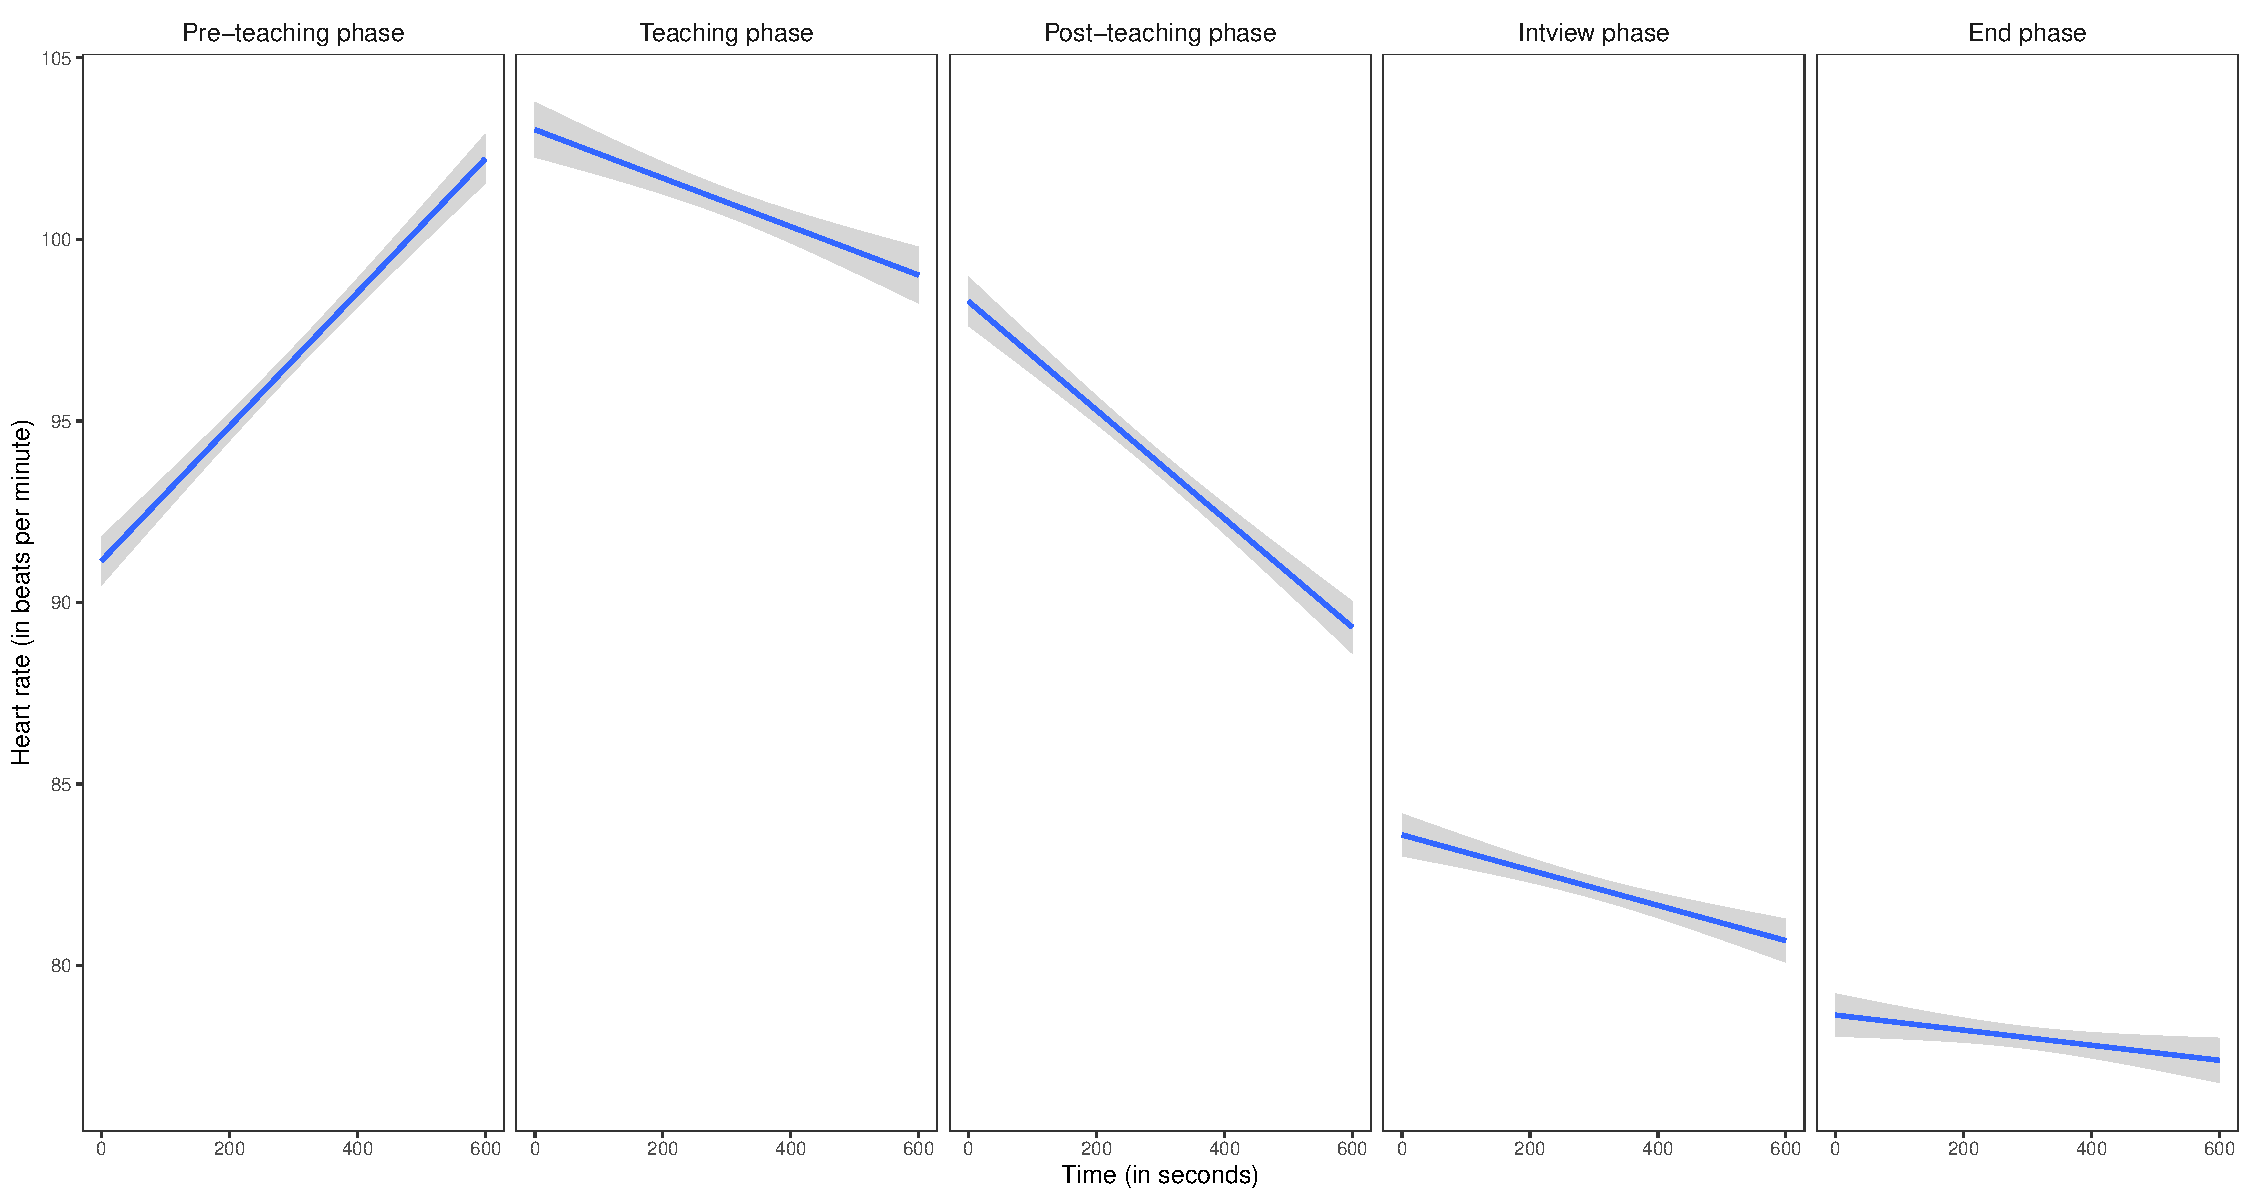
\includegraphics{fitbit_paper_files/figure-latex/phase_plot-1.pdf}

\hypertarget{discussion-and-implications}{%
\section{Discussion and implications}\label{discussion-and-implications}}

\newpage

\hypertarget{references}{%
\section{References}\label{references}}

\hypertarget{refs}{}
\begin{CSLReferences}{1}{0}
\leavevmode\vadjust pre{\hypertarget{ref-ALDRUP2018126}{}}%
Aldrup, K., Klusmann, U., Lüdtke, O., Göllner, R., \& Trautwein, U. (2018). Student misbehavior and teacher well-being: Testing the mediating role of the teacher-student relationship. \emph{Learning and Instruction}, \emph{58}, 126--136. https://doi.org/\url{https://doi.org/10.1016/j.learninstruc.2018.05.006}

\leavevmode\vadjust pre{\hypertarget{ref-R-DescTools}{}}%
Andri et mult. al., S. (2022). \emph{{DescTools}: Tools for descriptive statistics}. Retrieved from \url{https://cran.r-project.org/package=DescTools}

\leavevmode\vadjust pre{\hypertarget{ref-R-ggthemes}{}}%
Arnold, J. B. (2021). \emph{Ggthemes: Extra themes, scales and geoms for 'ggplot2'}. Retrieved from \url{https://CRAN.R-project.org/package=ggthemes}

\leavevmode\vadjust pre{\hypertarget{ref-R-gridExtra}{}}%
Auguie, B. (2017). \emph{gridExtra: Miscellaneous functions for "grid" graphics}. Retrieved from \url{https://CRAN.R-project.org/package=gridExtra}

\leavevmode\vadjust pre{\hypertarget{ref-R-papaja}{}}%
Aust, F., \& Barth, M. (2020). \emph{{papaja}: {Prepare} reproducible {APA} journal articles with {R Markdown}}. Retrieved from \url{https://github.com/crsh/papaja}

\leavevmode\vadjust pre{\hypertarget{ref-R-tinylabels}{}}%
Barth, M. (2022). \emph{{tinylabels}: Lightweight variable labels}. Retrieved from \url{https://cran.r-project.org/package=tinylabels}

\leavevmode\vadjust pre{\hypertarget{ref-R-lme4}{}}%
Bates, D., Mächler, M., Bolker, B., \& Walker, S. (2015). Fitting linear mixed-effects models using {lme4}. \emph{Journal of Statistical Software}, \emph{67}(1), 1--48. \url{https://doi.org/10.18637/jss.v067.i01}

\leavevmode\vadjust pre{\hypertarget{ref-R-Matrix}{}}%
Bates, D., Maechler, M., \& Jagan, M. (2022). \emph{Matrix: Sparse and dense matrix classes and methods}. Retrieved from \url{https://CRAN.R-project.org/package=Matrix}

\leavevmode\vadjust pre{\hypertarget{ref-Battipaglia2015}{}}%
Battipaglia, I., \& Lanza, G. A. (2015). The autonomic nervous system of the heart. In R. H. J. A. Slart, R. A. Tio, P. H. Elsinga, \& M. Schwaiger (Eds.), \emph{Autonomic innervation of the heart: Role of molecular imaging} (pp. 1--12). Berlin, Heidelberg: Springer Berlin Heidelberg. \url{https://doi.org/10.1007/978-3-662-45074-1_1}

\leavevmode\vadjust pre{\hypertarget{ref-R-lm.beta}{}}%
Behrendt, S. (2022). \emph{Lm.beta: Add standardized regression coefficients to lm-objects}. Retrieved from \url{https://CRAN.R-project.org/package=lm.beta}

\leavevmode\vadjust pre{\hypertarget{ref-claessens2017positive}{}}%
Claessens, L. C., Tartwijk, J. van, Want, A. C. van der, Pennings, H. J., Verloop, N., Brok, P. J. den, \& Wubbels, T. (2017). Positive teacher--student relationships go beyond the classroom, problematic ones stay inside. \emph{The Journal of Educational Research}, \emph{110}(5), 478--493.

\leavevmode\vadjust pre{\hypertarget{ref-donker2018quantitative}{}}%
Donker, M. H., Van Gog, T., \& Mainhard, M. T. (2018). A quantitative exploration of two teachers with contrasting emotions: Intra-individual process analyses of physiology and interpersonal behavior. \emph{Frontline Learning Research}, \emph{6}(3), 162--184.

\leavevmode\vadjust pre{\hypertarget{ref-doring2016empirische}{}}%
Döring, N., \& Bortz, J. (2016). Empirische sozialforschung im {Ü}berblick. In \emph{Forschungsmethoden und evaluation in den sozial-und humanwissenschaften} (pp. 3--30). Springer.

\leavevmode\vadjust pre{\hypertarget{ref-eid2015statistik}{}}%
Eid, M., Gollwitzer, M., \& Schmitt, M. (2015). \emph{Statistik und forschungsmethoden: Mit online-materialien (4., {ü}berarb. Und erw. aufl.)}. Weinheim: Beltz. Retrieved from https://contentselect. com/media/moz\_viewer~\ldots.

\leavevmode\vadjust pre{\hypertarget{ref-ertzberger2016use}{}}%
Ertzberger, J., \& Martin, F. (2016). Use of fitness bands by teachers in the classroom. \emph{TechTrends}, \emph{60}(4), 392--397.

\leavevmode\vadjust pre{\hypertarget{ref-ferguson2015validity}{}}%
Ferguson, T., Rowlands, A. V., Olds, T., \& Maher, C. (2015). The validity of consumer-level, activity monitors in healthy adults worn in free-living conditions: A cross-sectional study. \emph{International Journal of Behavioral Nutrition and Physical Activity}, \emph{12}(1), 1--9.

\leavevmode\vadjust pre{\hypertarget{ref-R-janitor}{}}%
Firke, S. (2021). \emph{Janitor: Simple tools for examining and cleaning dirty data}. Retrieved from \url{https://CRAN.R-project.org/package=janitor}

\leavevmode\vadjust pre{\hypertarget{ref-R-polycor}{}}%
Fox, J. (2022). \emph{Polycor: Polychoric and polyserial correlations}. Retrieved from \url{https://CRAN.R-project.org/package=polycor}

\leavevmode\vadjust pre{\hypertarget{ref-fuller2020reliability}{}}%
Fuller, D., Colwell, E., Low, J., Orychock, K., Tobin, M. A., Simango, B., et al.others. (2020). Reliability and validity of commercially available wearable devices for measuring steps, energy expenditure, and heart rate: Systematic review. \emph{JMIR mHealth and uHealth}, \emph{8}(9), e18694.

\leavevmode\vadjust pre{\hypertarget{ref-R-viridis}{}}%
Garnier, Simon, Ross, Noam, Rudis, Robert, \ldots{} Cédric. (2021a). \emph{{viridis} - colorblind-friendly color maps for r}. \url{https://doi.org/10.5281/zenodo.4679424}

\leavevmode\vadjust pre{\hypertarget{ref-R-viridisLite}{}}%
Garnier, Simon, Ross, Noam, Rudis, Robert, \ldots{} Cédric. (2021b). \emph{{viridis} - colorblind-friendly color maps for r}. \url{https://doi.org/10.5281/zenodo.4679424}

\leavevmode\vadjust pre{\hypertarget{ref-gold2015development}{}}%
Gold, B., \& Holodynski, M. (2015). Development and construct validation of a situational judgment test of strategic knowledge of classroom management in elementary schools. \emph{Educational Assessment}, \emph{20}(3), 226--248.

\leavevmode\vadjust pre{\hypertarget{ref-R-lubridate}{}}%
Grolemund, G., \& Wickham, H. (2011). Dates and times made easy with {lubridate}. \emph{Journal of Statistical Software}, \emph{40}(3), 1--25. Retrieved from \url{https://www.jstatsoft.org/v40/i03/}

\leavevmode\vadjust pre{\hypertarget{ref-helmke2014unterrichtsdiagnostik}{}}%
Helmke, A., Helmke, T., Lenske, G., Pham, G., Praetorius, A.-K., Schrader, F.-W., \& AdeThurow, M. (2014). Unterrichtsdiagnostik mit EMU. \emph{Aus-Und Fortbildung Der Lehrkr{ä}fte in Hinblick Auf Verbesserung Der Diagnosef{ä}higkeit, Umgang Mit Heterogenit{ä}t Und Individuelle F{ö}rderung}, 149--163.

\leavevmode\vadjust pre{\hypertarget{ref-R-purrr}{}}%
Henry, L., \& Wickham, H. (2020). \emph{Purrr: Functional programming tools}. Retrieved from \url{https://CRAN.R-project.org/package=purrr}

\leavevmode\vadjust pre{\hypertarget{ref-R-msm}{}}%
Jackson, C. H. (2011). Multi-state models for panel data: The {msm} package for {R}. \emph{Journal of Statistical Software}, \emph{38}(8), 1--29. Retrieved from \url{https://www.jstatsoft.org/v38/i08/}

\leavevmode\vadjust pre{\hypertarget{ref-R-ggpubr}{}}%
Kassambara, A. (2020). \emph{Ggpubr: 'ggplot2' based publication ready plots}. Retrieved from \url{https://CRAN.R-project.org/package=ggpubr}

\leavevmode\vadjust pre{\hypertarget{ref-R-rstatix}{}}%
Kassambara, A. (2021). \emph{Rstatix: Pipe-friendly framework for basic statistical tests}. Retrieved from \url{https://CRAN.R-project.org/package=rstatix}

\leavevmode\vadjust pre{\hypertarget{ref-R-needs}{}}%
Katz, J. (2016). \emph{Needs: Attaches and installs packages}. Retrieved from \url{https://CRAN.R-project.org/package=needs}

\leavevmode\vadjust pre{\hypertarget{ref-R-ppcor}{}}%
Kim, S. (2015). \emph{Ppcor: Partial and semi-partial (part) correlation}. Retrieved from \url{https://CRAN.R-project.org/package=ppcor}

\leavevmode\vadjust pre{\hypertarget{ref-kyriacou2001teacher}{}}%
Kyriacou, C. (2001). Teacher stress: Directions for future research. \emph{Educational Review}, \emph{53}(1), 27--35.

\leavevmode\vadjust pre{\hypertarget{ref-R-jtools}{}}%
Long, J. A. (2022). \emph{Jtools: Analysis and presentation of social scientific data}. Retrieved from \url{https://cran.r-project.org/package=jtools}

\leavevmode\vadjust pre{\hypertarget{ref-lowe2016educational}{}}%
Lowe, H. (2016). Educational behavior apps and wearable devices: Current research and prospects. \emph{Educational Technology}, 30--33.

\leavevmode\vadjust pre{\hypertarget{ref-lu2008can}{}}%
Lu, S., Zhao, H., Ju, K., Shin, K., Lee, M., Shelley, K., \& Chon, K. H. (2008). Can photoplethysmography variability serve as an alternative approach to obtain heart rate variability information? \emph{Journal of Clinical Monitoring and Computing}, \emph{22}(1), 23--29.

\leavevmode\vadjust pre{\hypertarget{ref-R-imputeTS}{}}%
Moritz, S., \& Bartz-Beielstein, T. (2017). {imputeTS: Time Series Missing Value Imputation in R}. \emph{{The R Journal}}, \emph{9}(1), 207--218. \url{https://doi.org/10.32614/RJ-2017-009}

\leavevmode\vadjust pre{\hypertarget{ref-R-tibble}{}}%
Müller, K., \& Wickham, H. (2021). \emph{Tibble: Simple data frames}. Retrieved from \url{https://CRAN.R-project.org/package=tibble}

\leavevmode\vadjust pre{\hypertarget{ref-R-base}{}}%
R Core Team. (2022). \emph{R: A language and environment for statistical computing}. Vienna, Austria: R Foundation for Statistical Computing. Retrieved from \url{https://www.R-project.org/}

\leavevmode\vadjust pre{\hypertarget{ref-R-ltm}{}}%
Rizopoulos, D. (2006). Ltm: An r package for latent variable modelling and item response theory analyses. \emph{Journal of Statistical Software}, \emph{17}(5), 1--25. Retrieved from \url{https://doi.org/10.18637/jss.v017.i05}

\leavevmode\vadjust pre{\hypertarget{ref-R-broom}{}}%
Robinson, D., Hayes, A., \& Couch, S. (2022). \emph{Broom: Convert statistical objects into tidy tibbles}. Retrieved from \url{https://CRAN.R-project.org/package=broom}

\leavevmode\vadjust pre{\hypertarget{ref-rungeusing}{}}%
Runge, N., Haarman, S., \& Fisher, M. H. (n.d.). \emph{Using fitbit fitness trackers to measure teacher stress and coping}.

\leavevmode\vadjust pre{\hypertarget{ref-sachs2014physiologische}{}}%
Sachs, S. (2014). \emph{Physiologische parameter zur bewertung der lernwirksamkeit von lernsituationen} (PhD thesis). Universit{ä}t Ulm.

\leavevmode\vadjust pre{\hypertarget{ref-R-MASS}{}}%
Venables, W. N., \& Ripley, B. D. (2002). \emph{Modern applied statistics with s} (Fourth). New York: Springer. Retrieved from \url{https://www.stats.ox.ac.uk/pub/MASS4/}

\leavevmode\vadjust pre{\hypertarget{ref-wang2022using}{}}%
Wang, C., Lizardo, O., \& Hachen, D. S. (2022). Using fitbit data to monitor the heart rate evolution patterns of college students. \emph{Journal of American College Health}, \emph{70}(3), 875--882.

\leavevmode\vadjust pre{\hypertarget{ref-R-ggplot2}{}}%
Wickham, H. (2016). \emph{ggplot2: Elegant graphics for data analysis}. Springer-Verlag New York. Retrieved from \url{https://ggplot2.tidyverse.org}

\leavevmode\vadjust pre{\hypertarget{ref-R-stringr}{}}%
Wickham, H. (2019). \emph{Stringr: Simple, consistent wrappers for common string operations}. Retrieved from \url{https://CRAN.R-project.org/package=stringr}

\leavevmode\vadjust pre{\hypertarget{ref-R-forcats}{}}%
Wickham, H. (2021). \emph{Forcats: Tools for working with categorical variables (factors)}. Retrieved from \url{https://CRAN.R-project.org/package=forcats}

\leavevmode\vadjust pre{\hypertarget{ref-R-tidyverse}{}}%
Wickham, H., Averick, M., Bryan, J., Chang, W., McGowan, L. D., François, R., \ldots{} Yutani, H. (2019). Welcome to the {tidyverse}. \emph{Journal of Open Source Software}, \emph{4}(43), 1686. \url{https://doi.org/10.21105/joss.01686}

\leavevmode\vadjust pre{\hypertarget{ref-R-readxl}{}}%
Wickham, H., \& Bryan, J. (2022). \emph{Readxl: Read excel files}. Retrieved from \url{https://CRAN.R-project.org/package=readxl}

\leavevmode\vadjust pre{\hypertarget{ref-R-dplyr}{}}%
Wickham, H., François, R., Henry, L., \& Müller, K. (2022). \emph{Dplyr: A grammar of data manipulation}. Retrieved from \url{https://CRAN.R-project.org/package=dplyr}

\leavevmode\vadjust pre{\hypertarget{ref-R-tidyr}{}}%
Wickham, H., \& Girlich, M. (2022). \emph{Tidyr: Tidy messy data}. Retrieved from \url{https://CRAN.R-project.org/package=tidyr}

\leavevmode\vadjust pre{\hypertarget{ref-R-readr}{}}%
Wickham, H., Hester, J., \& Bryan, J. (2022). \emph{Readr: Read rectangular text data}. Retrieved from \url{https://CRAN.R-project.org/package=readr}

\leavevmode\vadjust pre{\hypertarget{ref-R-cowplot}{}}%
Wilke, C. O. (2020). \emph{Cowplot: Streamlined plot theme and plot annotations for 'ggplot2'}. Retrieved from \url{https://CRAN.R-project.org/package=cowplot}

\leavevmode\vadjust pre{\hypertarget{ref-R-xfun}{}}%
Xie, Y. (2022). \emph{Xfun: Supporting functions for packages maintained by 'yihui xie'}. Retrieved from \url{https://CRAN.R-project.org/package=xfun}

\end{CSLReferences}


\end{document}
